\documentclass[a4paper]{article} % article class, paper size A4
\usepackage{lipsum} 	% add package for dummy texts
\usepackage{amsmath}	% For math
\usepackage{graphicx}	% For extra setting for figures
\usepackage{hyperref}	% To make clickable hyperlinks
\usepackage{cleveref}	% To make smart references
\usepackage{float}		% For easier and more precise placement

\setlength{\parindent}{0pt}

\renewcommand{\figurename}{Fig.}
\renewcommand{\tablename}{Table}

%%%%% Bibliography settings
\usepackage[backend=biber, style=IEEE]{biblatex} % Style of the bibliography (IEEE)
\addbibresource{./library.bib}	% Location of the bibliography file

\author{Name} % author of the document
\title{Title} % title/Name of the document
\date{\today} % date with current date

\begin{document} % start document

%%% Need to write some text
% Test

\maketitle % Create title page
\pagebreak % whatever comes next: be on the next page
\tableofcontents % create a table of contents
\pagebreak % see above

\section*{Epilogue} % unnumbered header (*) lvl 1
\lipsum[1] % create some dummy text

\section{Introduction} % numbered header lvl 1
\lipsum[2-4]

\section{Methodology} % numbered header lvl 1
\lipsum[1-3]

\subsection{First subsection} % numbered header under previous header, lvl 1.1
\lipsum[1]

\clearpage

This line has an indentation.\\
This line will not have an indentation because it is still part of the same paragraph.

What about this sentence?\\

\noindent This sentence for sure will have no indent.\\

Or we can use the function \verb|\setlength{\parindent}{0pt}| at the beginnign of the document to have no indentation anywhere!\\

\hrulefill

This is an inline math equation: $a^2 + b^2 = c^2$ and it has no numbering.

\begin{align}
E &= mc^2            	&& Einstein's equations \label{eq:einstein}     	\\
a^2 + b^2 &= c^2     && Pythagoras' equation \label{eq:pythagoras}		\\
\frac{\partial \mathcal D}{t} &= \Delta \times \mathcal H	&& Faraday's Law \label{eq:faraday}
\end{align}

With standard \LaTeX, the references look like this:\\
This is \ref{eq:einstein}, and \ref{eq:pythagoras}, but what I actually wanted was something like this: This is eqn. \ref{eq:einstein} and this is eqn. \ref{eq:pythagoras}.\\
But who wants to type this all the time? Not me!

I will use another package, such as 'Cleveref', then the first equation is \cref{eq:einstein} and second equation is \cref{eq:pythagoras}.\\
I can also call several equations such as \crefrange{eq:einstein}{eq:faraday} or \crefrange*{eq:einstein}{eq:pythagoras} or \crefrange*{eq:pythagoras}{eq:faraday}
\\

\hrulefill\\

Now I will show how to add a table with TexMaker:



\hrulefill\\

Now I will show how to add an image:
Do you want to know how Einstein looks like?\\

\begin{figure}[H] %[H]
	\center
	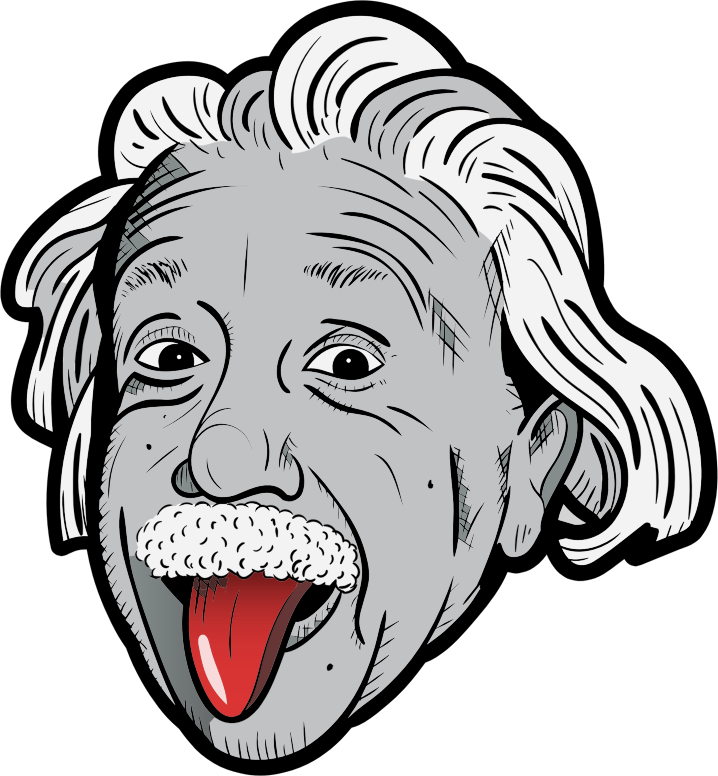
\includegraphics[width=0.8\textwidth]{./img/einstein.png}
	\caption{Famous picture of Einstein}
	\label{fig:einstein}
\end{figure}

Have a look at \ref{fig:einstein} or I use Cleveref again: \cref{fig:einstein}.\\
We see again that it doesn't add 'Fig.' before the reference. If we don't like that the caption under the figure starts with "Figure" we can add at the beginning of the document this code: \verb|\renewcommand{\figurename}{Fig.}| and it will automatically change the text for us.\\
He wrote the famous equation (\cref{eq:einstein}) in 1919 in his paper \cite{Einstein1919}.

\newpage

% \section{References}
\addcontentsline{toc}{section}{References}
\printbibliography

\end{document} % end of document